\section{Methoden zur Feature-Auswahl, Hyperparametersuche und Modellauswahl} \label{sec:Meth FeatHypModSelect}
Zwischen der Feature-Auswahl, Modellauswahl und Hyperparametersuche besteht ein enger Zusammenhang. Werden für die Feature-Auswahl modellabhängige Methoden verwendet, wie die Wrapper-Methoden, muss ein Modell vorhanden sein, mit dem sie durchgeführt werden können. Für die Wahl zwischen unterschiedlichen Modellen auf Basis ihrer Performance sowie eine faire Bewertung ist eine Einstellung der Hyperparameter notwendig. Ein Modell \(A\) wird beispielsweise mit einem Modell \(B\) verglichen. Die Hyperparameter sind noch nicht eingestellt. Modell \(A\) erzielt eine bessere Performance. Anschließend werden passende Hyperparameter gesucht, bevor ein weiterer Vergleich nun Modell \(B\) als bessere Wahl ausweist. \par

Um also ein möglichst effektives Modell zu erhalten, ist eine grobe Voreinstellung der Hyperparameter der Modelle durchzuführen. Anschließend wird eine Methode für die Feature-Auswahl angewendet. Da die Modelle vorhanden und eingestellt sind, darf diese modellabhängig oder modellunabhängig sein. Im Anschluss kann die Performance der Modelle verglichen werden. Das Beste wird ausgewählt und eine Feineinstellung der Hyperparameter wird durchgeführt. Darauf folgt final die Überprüfung mittels Testdatensatz, bevor das Modell für den Einsatz bereit ist.\par

Da die Hyperparametersuche über die Optimierung des Validierungsergebnisses geschieht und dafür Modelle trainiert werden müssen, bedarf es hier bereits guter Features. Aus diesem Grund wird eine Vorauswahl der Features durchgeführt, um die Menge einzugrenzen. Da uninformative Features Underfitting und redundante Features Overfitting provozieren können, ist eine Vorauswahl sinnvoll, um eine aussagekräftige Einschätzung der Generalisierfähigkeit der Modelle zu erhalten. \par

Wie in \autoref{sec:Meth Datensatz} dargestellt, wird aufgrund der begrenzten Datenmenge für die Validierung Cross-Validation angewendet (\autoref{sec:ML Metriken, Valid}). Für das Training und das Testen wird der Datensatz aus \autoref{tab:DataNachBalance} in einen Trainingsdatensatz und einen Testdatensatz aufgeteilt. Von der Datenmenge werden 20 \% für das Testen beiseitegelegt. Die Tabelle \ref{tab:TrainTestSplit} zeigt die Datenmengen, die für Training und Testen zur Verfügung stehen.


\begin{table}[ht]
    \centering
    \caption{Aufteilung der Daten in Trainings- und Testdatensatz.}
    \begin{tabular}{|l|r|r|}
        \hline
        Datensatz & Datenmenge & Anteil \\
        \hline
        Trainingsdatensatz & 528 & 80 \%\\
        Testdatensatz & 132 & 20 \%\\
        \hline
        \hline
        Gesamt & 660 & 100 \%\\
        \hline
    \end{tabular}
    \label{tab:TrainTestSplit}
\end{table}

\subsection{Vorauswahl der Features} \label{sec:Meth FeatVorSele}
Aufgrund ihrer Modellunabhängigkeit werden zunächst die Filter-Methoden angewendet. Dadurch entstehen  Feature Rangfolgen: eine für die Varianzanalyse und eine für die gegenseitige Information. Jedoch ist die Qualität dieser Rangfolgen nicht überprüfbar, ohne Modell, da sonst keine Performance ermittelt werden kann. Aus diesem Grund wurde sich ein Verfahren überlegt, wie die Rangfolge der Filter-Methoden möglichst modellunabhängig evaluiert werden kann. \par

Als Beispiel wird ein Modell wie die logistische Regression herangezogen, das unkonfiguriert bleibt. Es wird mit den Standardeinstellungen der \gls{Bibliothek} angewendet. Gemäß der Rangfolge bekommt das Modell inkrementell die Features übergeben, wobei es in jeder Inkrementation trainiert und validiert wird. In der ersten Inkrementation wird das Modell also nur mit dem höchstrangigen Feature aufgebaut, in der zweiten Inkrementation mit den beiden höchstrangigen Features und in der dritten mit den drei höchstrangigen Features. Validiert werden die Modelle mit der Metrik Accuracy und Cross-Validation. Somit entsteht ein Verlauf, der sich zweidimensional visualisieren lässt. Auf der y-Achse wird die Accuracy dargestellt und auf der y-Achse die Feature-Anzahl, mit der das jeweilige Modell trainiert wurde. Die Abbildung \ref{fig:bspSättAccu} zeigt beispielhaft einen Linienplot der Accuracy. 

\begin{figure}[htb]
    \centering
    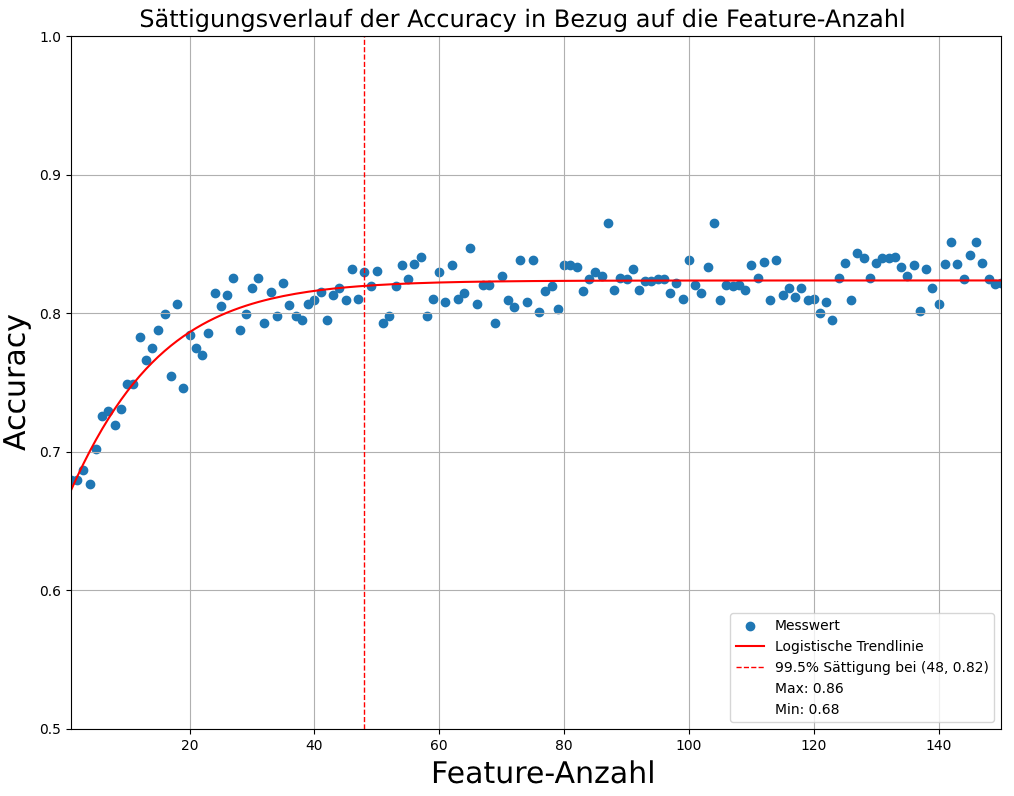
\includegraphics[width=0.9\textwidth]{img/Plots/bsp Accuracy verlauf.png}
    \caption[Beispiel eines Verlaufs der Accuracy in Bezug auf die Feature-Anzahl.]{Beispiel eines Verlaufs der Accuracy in Bezug auf die Feature-Anzahl, für die Feature-Vorauswahl. Die Accuracy verläuft in eine Sättigung.}
    \label{fig:bspSättAccu}
\end{figure}

Die resultierende Betrachtung lässt eine grafische Beurteilung der Feature-Auswahl zu. Auch multivariate Einflüsse werden hier angezeigt. Jedoch ist das Vorgehen noch modellabhängig. Um die Ergebnisse zu verallgemeinern, wird der Verlauf der Accuracy für jedes Modell in der Vorauswahl gemessen. Die Werte werden anschließend gemittelt. Dadurch entsteht ein Verlauf der Accuracy, der sich nicht auf ein bestimmtes Modell bezieht. Die Methode ist also verwendbar, um eine Feature-Rangfolge möglichst modellunabhängig zu beurteilen.\par

Wichtig zu erwähnen ist, dass die Feature-Werte für eineiige Modelle skaliert werden müssen, damit diese mit den Features arbeiten können. Für die lineare Regression werden diese auf den Wertebereich [0;1] skaliert. Für die SVMs werden alle Features auf den Wertebereich [-1;1] skaliert.\par

Wie in der Abbildung \ref{fig:bspSättAccu} zu sehen ist, verläuft die Genauigkeit in eine Sättigung. Ein solcher Verlauf zeigte sich bei allen durchgeführten Versuchen. Da die Messwerte schwanken, wird der Verlauf mit einer Sättingungslinie approximiert. Somit steht ein stabileres Maß für die Beurteilung und für Vergleiche zur Verfügung. Der Sättigungsverlauf deutet auf Redundanzen in den Features hin. Ab einer bestimmten Feature-Menge erhält das Modell keine neuen Informationen durch weitere Features. Das ist nicht verwunderlich, da alle Features auf den 38 Basis-Features aufbauen. Der Sättigungsverlauf ist praktisch für die Feature-Auswahl, da über den Punkt, an dem die Sättigung erreicht wird, eine optimale Feature-Menge bestimmt ist. \par

Da die Rangfolge der Filter-Methoden, wie bereits erwähnt, durch eine univariate Beurteilung erfolgt, ist zu vermuten, dass sie nicht optimal ist. Eine Rangfolge, die die Features multivariat beurteilt, ist wünschenswert. Mit den Wrapper-Methoden lassen sich Features auswählen, da sie als Verfahren auch multivariate Zusammenhänge berücksichtigen. Die Wrapper-Methoden erstellen jedoch keine Rangfolge. Es werden deshalb mehrere Messreihen aufgenommen. Die Ergebnisse der Messreihen sollen in eine Rangfolge der Features überführt werden.\par

Aus der Anwendung der Wrapper-Methoden auf ein Modell und eine Feature-Menge ist eine binäre Wertung eines Features abzuleiten: \textit{ausgewählt} oder \textit{nicht ausgewählt}. Werden mehrere Wiederholungen durchgeführt, in denen die Wrapper Methoden angewendet werden, bei denen die Zusammensetzung der Feature-Menge variiert wird und auch das Modell, so entstehen mehrere binäre Evaluationen eines Features. Aus diesen kann eine Gesamtwertung des Features abgeleitet werden. Die Tabelle \ref{tab:bspWrapScore} veranschaulicht dies an einem Beispiel und die Formel \ref{eq:Meth WrapperScore} zeigt die Berechnung der Wertung.

\begin{table}[htb]
    \centering
    \caption{Beispiel einer Versuchsreihe zu dem Feature i, durch die Anwendung von Wrapper-Methoden.}
    \begin{tabular}{|c|r|r|}
        \hline
        \multicolumn{3}{|r|}{\(Feature_i\)} \\
        \hline
        Versuch ID & ausgewählt & nicht ausgewählt \\
        \hline
        0 & 1 & 0 \\
        1 & 1 & 0 \\
        2 & 0 & 1 \\
        3 & 1 & 0 \\
        4 & 0 & 1 \\
        5 & 1 & 0 \\
        \hline
        \hline
        Gesamt & 4 & 2 \\
        \hline
    \end{tabular}
    \label{tab:bspWrapScore}
\end{table}

\begin{equation}
W(x) = \frac{|\text{Ausgewählt}(x)|}{|\text{ausgewählt}(x)| + |\text{nicht ausgewählt}(x)|} \rightarrow W(Feature_i)=\frac{4}{4+2} = 67\ \%
\label{eq:Meth WrapperScore}
\end{equation}

In der Formel \ref{eq:Meth WrapperScore} ist \(W(x)\) die Wertung eines Features \(x\). Zur Klarheit wird \(w\) im Folgenden als \textit{Wrapper-Score} bezeichnet. Der Mechanismus des Wrapper-Scores ist einfach. Wird ein Feature auch in unterschiedlichen Feature-Mengen und von verschiedenen Modellen oft ausgewählt, steigt der Wert. Das Maximum ist 1 und das Minimum 0. Features, die in Kombination miteinander informativ sind, werden in der Hinsicht berücksichtigt, dass diese einen ähnlichen Wrapper-Score erzielen sollten. Sind sie sehr informativ, stehen sie gemeinsam weit oben in der Rangfolge. \par

Um eine aussagekräftige Rangfolge durch die Wrapper-Scores zu erhalten, sind Messreihen aufzunehmen. Dazu sind mehrere Modelle zu benutzen. Verwendet werden eine klassische logistische Regression, eine lineare SVM und ein Random Forest Modell, ein histogrammbasiertes Gradient Boosting und eine polynomiale SVM. Die polynomiale SVM kann eine polynomiale Entscheidungsebene modellieren. Sie ist auf eine Polynomfunktion dritter Ordnung eingestellt. Die Feature-Mengen werden variiert, indem unterschiedliche Kombinationen der Oberkategorien der Features (\autoref{tab:FeatureMenge}) in die Modelle gegeben werden. Eine Variation der Zusammensetzung der Feature-Menge durch zufälliges Ziehen aus der Gesamtmenge würde mehr Varianz bringen, jedoch ist das Durchführen der Versuche zeitaufwendig. Um zu garantieren, dass jedes Feature in einer praktikablen Zeit betrachtet wird, wird sich für den beschriebenen Ansatz entschieden.\par

Wie in \autoref{sec:ML FeatSelect} veranschaulicht, gibt es für die Anwendung der Wrapper-Methoden mehrere Verfahren. Um auch hier für Varianz zu sorgen, werden Messreihen aufgenommen, mit der Vorwärtsauswahl und der Rückwärtsauswahl. Auch die Kriterien, nach denen ausgewählt wird, werden variiert. In einigen Messreihen soll eine bestimmte Anzahl an Features ausgewählt werden und in anderen Messreihen, sollen so viele Features ausgewählt werden, bis die Performance nicht mehr steigt. Eine Übersicht über die durchgeführten Versuche befindet sich im Anhang. Sind bestimmte Versuche nicht mit gewissen Feature-Kategorien oder Modellen durchgeführt worden, lag dies am Rechenaufwand. Insgesamt wurden 179 unterschiedliche Kombinationen von Feature-Mengen, Wrapper-Methoden und Modellen getestet. \par

Aus diesen Versuchen lässt sich für jedes Feature ein Wrapper-Score ermitteln und eine Rangfolge der Features ist erstellbar. Die Rangfolge kann modellunabhängig über den Plot der Accuracy evaluiert werden, wie in \autoref{fig:bspSättAccu} vorgeführt wird. \par

Prädestiniert für Redundanz sind Features, die sich die gleiche Basis teilen. Wie zum Beispiel die maximale Geschwindigkeit einer Trajektorie, welche sowohl in ihrer Basisform vorliegt als auch als Quantil-Feature. Ist eine Feature-Basis sehr informativ, ist es nicht unwahrscheinlich, dass mehrere Features, die sich diese Basis teilen, einen hohen Rang erzielen und Redundanz in der Feature-Auswahl entsteht. Um das zu reduzieren, wird lediglich das höchstrangige Feature der gleichen Basis in der Rangfolge behalten. Features mit gleicher Basis, aber mit einem niedrigeren Rang,  werden aus der Rangfolge entfernt. Interaktionsfeatures stellen dabei ihre eigene Basis dar. Die Kombination aus maximaler Geschwindigkeit und der mittleren Objektanzahl teilt sich bei dieser Methode nicht die gleiche Basis wie die maximale Geschwindigkeit und auch nicht wie die mittlere Objektanzahl. Anderes gilt für die Interaktion mit sich selbst. \par

Die Evaluation bestätigt, dass durch das Eliminieren von Features mit gleicher Basis eine effizientere Rangfolge entsteht. Die Sättigung wird früher erreicht. In \autoref{sec:Ergeb FeatSel,Hyp,ModSel} wird dies genauer dargestellt. \par

Abschließend wird untersucht, ob alle Feature-Kategorien benötigt werden. Dazu werden aus der Rangfolge nur Features aus bestimmten Kategorien genommen und evaluiert. Im \autoref{sec:Ergeb FeatKategories} befindet sich eine tabellarische Übersicht über die durchgeführten Versuche. \par

Bei der Auswertung in \autoref{sec:Ergeb FeatSel,Hyp,ModSel} zeigt sich, dass mit der Zusammensetzung der Feature-Menge aus Basis-Features, Interaktionsfeatures und Quantil-Features die besten Ergebnisse erzielt werden. Die Box-Cox-Features und die Logarithmus-Features werden aus der Vorauswahl herausgenommen. \par

Mit der resultierenden Rangfolge wird mit 29 Features die Sättigung der Accuracy erreicht. Um die Menge der Features in der Vorauswahl nicht zu sehr zu beschneiden, werden die besten 150 Features der Rangfolge als Vorauswahl gewählt. 



\subsection{Einstellung der Hyperparameter} \label{sec:Meth HyperparaKonf}
Für die zur Auswahl stehenden Modelle sind passende Hyperparameter zu finden. Dafür verwendet werden die 150 Features der Vorauswahl. Für die Hyperparametersuche wird eine Random Search durchgeführt (\autoref{sec:ML HyperPara}). Unternommene Versuche, die Grid Search anzuwenden zeigten, dass diese zu viel Rechenzeit benötigt. Eingestellt werden die folgenden Modelle:

\begin{enumerate}
    \item Logistische Regression
    \item Lineare SVM
    \item Polynomiale SVM
    \item Random Forest
    \item Gradient Boosting
    \item Histogramm basiertes Gradient Boosting
\end{enumerate}

Insgesamt werden für jedes Modell 500 Kombinationen von Hyperparametern getestet. Diese werden mittels Cross-Validation beurteilt. Da in vorherigen Tests bemerkt wurde, dass die Accuracy schwanken kann, wurde jede Kombination 150 Mal validiert. Trotz des Aufwands ist dieser nötig, da es das Ziel ist, eine statistische Stabilität der Accuracy zu erhalten. Nur wenn diese gegeben ist, kann der Aussage vertraut werden, dass eine bestimmte Kombination an Hyperparametern besser ist als eine andere. Die Schwankungen in der Accuracy sind vermutlich auf die geringe Datenmenge zurückzuführen. \par

Um die hohe Anzahl an Validierungswerten zu erhalten, wird eine mehrfache Cross-Validation durchgeführt. Insgesamt wird der Trainingsdatensatz in 10 Teile zerteilt, mit denen jeweils eine Validierung durchgeführt wird. Anschließend wird der Trainingsdatensatz neu durchmischt und die Cross-Validation wird wiederholt. Dies wird insgesamt 15 Mal wiederholt. \par

Die erzielte Accuracy und die dazugehörigen Hyperparameter werden abgespeichert. Nach Vollendung der Random Search können die Ergebnisse in eine Reihenfolge gebracht werden. Die Hyperparameter, mit denen die beste Performance erzielt wurde, werden für das Modell übernommen. \par

Informativ kann auch die Betrachtung der Hyperparameter der oberen Ränge sein, da diese ebenfalls eine hohe Accuracy erzielten und aufgrund ähnlicher Größenordnungen mit hoher Sicherheit gut eingestellt sind. Schwanken die Werte eines Hyperparameters stark, dann ist dieser entweder nicht relevant für die Lösung der Aufgabe oder es existieren Mehrdeutigkeiten in der Kombination mit anderen Hyperparametern. \par

Eine ausführliche Übersicht über die Hyperparameter der einzelnen Modelle und die Wahrscheinlichkeitsverteilungen, aus denen die Random Search die jeweiligen Parameterwerte zieht, befindet sich im Anhang. 

\subsection{Auswahl des Modells und der Features}\label{sec:Meth ModelSele}
Da nun die Modelle eingestellt sind und eine Feature-Vorauswahl vorhanden ist, ist die finale Entscheidung für ein Modell einfach. Für jedes eingestellte Modell wird der Verlauf der Accuracy in Bezug auf die Rangliste ermittelt, wie in \autoref{fig:bspSättAccu} beispielhaft dargestellt. Anschließend können die Verläufe verglichen werden. Das Modell, das die beste Performance zeigt, wird ausgewählt. Über den Sättigungspunkt ist eine optimale Feature-Menge direkt ablesbar. Erzielen zwei Modelle die gleiche Performance, wird das Modell bevorzugt, das diese mit der geringsten Feature-Menge erreicht. \par

Es zeigt sich, dass eine polynomiale SVM das beste Modell ist. Die Entscheidungsebene ist mit einer Funktion zweiten Grades modellierbar. Der Sättigungspunkt wird laut Trendlinie mit 18 Features erreicht. Um für mehr Stabilität tiefer in der Sättigung zu liegen, werden die besten 40 Features verwendet. Die polynomiale SVM implementiert keine Embedded-Methoden für die Feature-Auswahl, somit wird diese nicht weiter optimiert. \par

Abschließend wird das Modell trainiert und getestet. Der Test bestätigt das Modell, wie in \autoref{sec:Ergeb ModEntwi} dargestellt wird.\par

Im Anhang befindet sich eine Liste der ausgewählten Features. Ebenfalls sind dort die ermittelten Hyperparameter des finalen Modells tabellarisch aufgeführt.